\subsubsection{Caso d’uso UC8.1.3.5: Creazione domanda a ordinamento di immagini}
\label{UC8.1.3.5}
	\begin{figure}[h]
		\centering
			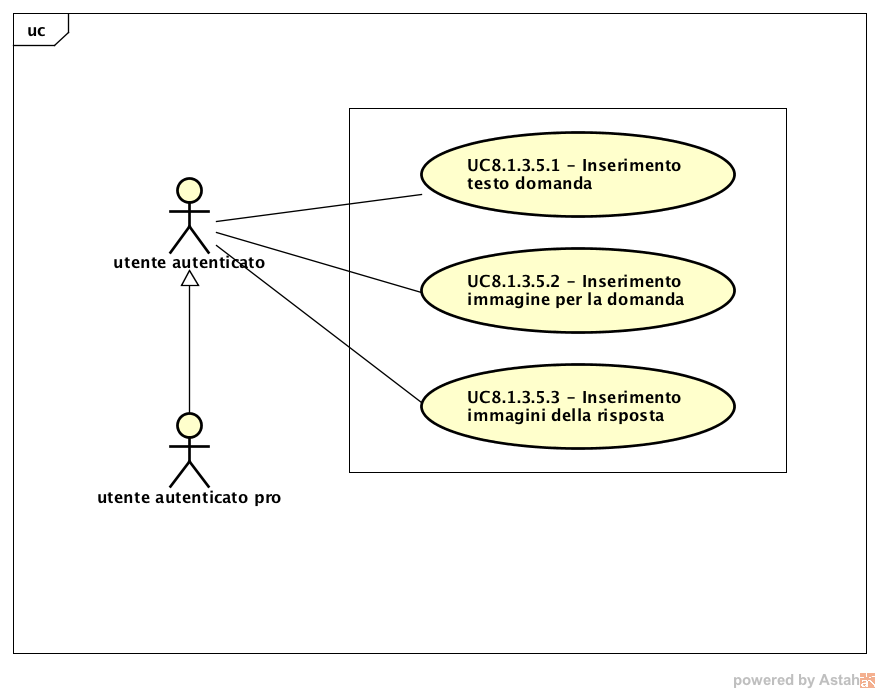
\includegraphics[scale=0.45,keepaspectratio]{UML/UC8_1_3_5.png}
		\caption{UC8.1.3.5: Creazione domanda a ordinamento immagini}
	\end{figure}
	\FloatBarrier
\begin{itemize}
	\item\textbf{Attori}: utente autenticato, utente autenticato pro;
	\item\textbf{Scopo e descrizione}: l'attore  possono inserire una domanda del tipo ordinamento di immagini;
	\item\textbf{Precondizione}: il sistema mostra all'attore  il form di inserimento dei campi dati per la tipologia di domanda scelta; 
	\item \textbf{Postcondizione}: l'attore ha inserito tutti i campi dati obbligatori;
	\item\textbf{Scenario principale}:
	\begin{itemize}
		\item Gli attori devono compilare il campo dati destinato alla scrittura del testo della domanda (UC8.1.3.5.1);
		\item Gli attoriinserisce un'immagine per il testo della domanda (UC8.1.3.5.2);
		\item Gli attori devono inserire le immagini nel giusto ordine (UC8.1.3.5.3).
	\end{itemize}
\end{itemize}

\subsubsection{Caso d’uso UC8.1.3.5.1: Inserimento testo domanda}
\begin{itemize}
	\item\textbf{Attori}: utente autenticato, utente autenticato pro;
	\item\textbf{Scopo e descrizione}: lo scopo di questa funzionalità è offrire all'attore  la possibilità di inserire il testo della domanda;
	\item\textbf{Precondizione}: l'attore ha scelto la modalità di creazione della domanda a ordinamento di immagini; 
	\item \textbf{Postcondizione}: l'attore ha inserito il testo della domanda;
	\item\textbf{Scenario principale}: l'attore  devono inserire il testo della domanda. 
\end{itemize}

\subsubsection{Caso d’uso UC8.1.3.5.2: Inserimento immagine per testo domanda}
\label{UC8.1.3.5.2}
\begin{figure}[h]
	\centering
	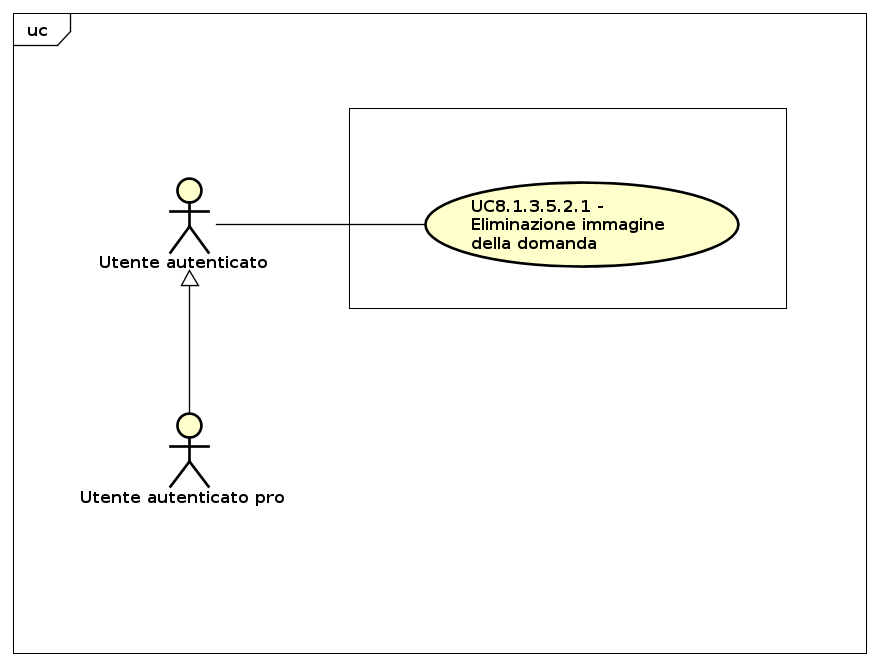
\includegraphics[scale=0.45,keepaspectratio]{UML/UC8_1_3_5_2.png}
	\caption{UC8.1.3.5.2: Inserimento immagine per testo domanda}
\end{figure}
\FloatBarrier
\begin{itemize}
	\item\textbf{Attori}: utente autenticato, utente autenticato pro;
	\item\textbf{Scopo e descrizione}: lo scopo di questa funzionalità è offrire all'attore  la possibilità di inserire un'immagine relativa domanda;
	\item\textbf{Precondizione}: l'attore ha scelto la modalità di creazione della domanda a ordinamento di immagini; 
	\item \textbf{Postcondizione}: l'attore ha inserito un'immagine relativa alla domanda;
	\item\textbf{Scenario principale}: 
		\begin{enumerate}
			\item L'attore inserisce un'immagine relativa alla domanda;
			\item L'attore può eliminare l'immagine appena inserita (UC8.1.3.5.2.1).
		\end{enumerate}

\end{itemize}

\subsubsection{Caso d’uso UC8.1.3.5.2.1: Eliminazione immagine per testo domanda}
\begin{itemize}
	\item\textbf{Attori}: utente autenticato, utente autenticato pro;
	\item\textbf{Scopo e descrizione}: lo scopo di questa funzionalità è offrire all'attore  la possibilità di rimuovere l'immagine relativa ad domanda appena inserita;
	\item\textbf{Precondizione}: l'attore ha scelto la modalità di eliminazione dell'immagine usata come testo; 
	\item \textbf{Postcondizione}: l'attore ha eliminato l'immagine relativa alla domanda;
	\item\textbf{Scenario principale}: l'attore rimuove l'immagine relativa alla domanda. 
\end{itemize}

\subsubsection{Caso d’uso UC8.1.3.5.3: Inserimento immagini della risposta}
\label{UC8.1.3.5.3}
\begin{figure}[h]
	\centering
	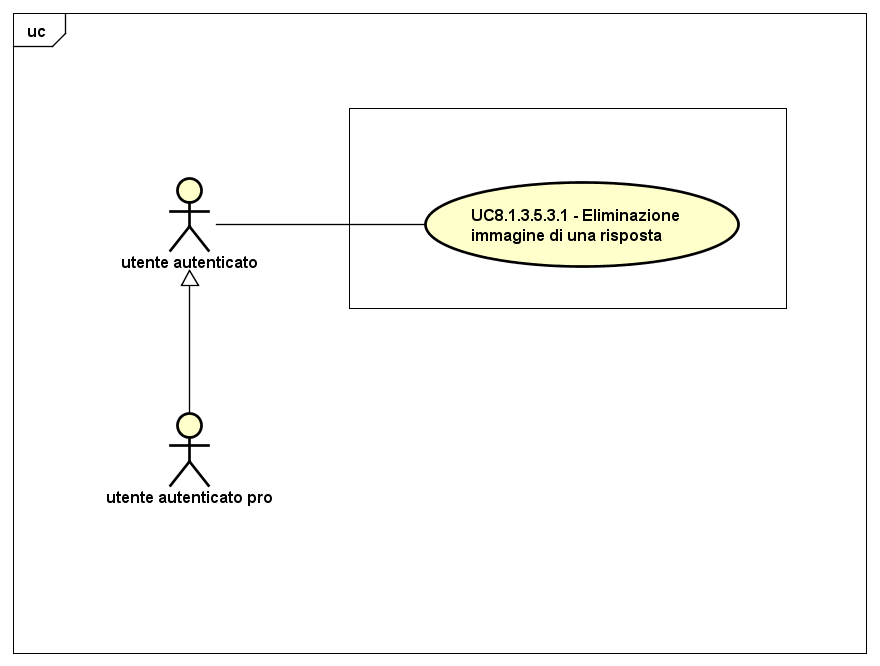
\includegraphics[scale=0.45,keepaspectratio]{UML/UC8_1_3_5_3.png}
	\caption{UC8.1.3.5.3: Inserimento immagini della risposta}
\end{figure}
\begin{itemize}
	\item\textbf{Attori}: utente autenticato, utente autenticato pro;
	\item\textbf{Scopo e descrizione}: lo scopo di questa funzionalità è offrire all'attore  la possibilità di inserire le immagini per la risposta della relativa domanda;
	\item\textbf{Precondizione}: l'attore ha scelto la modalità di creazione della domanda a ordinamento di immagini; 
	\item \textbf{Postcondizione}: l'attore ha inserito delle immagini in ordine corretto per la risposta relativa alla domanda;
	\item\textbf{Scenario principale}:
		\begin{enumerate}
			\item L''attore inserisce delle immagini in ordine corretto per la relativa domanda;
			\item L'attore può eliminare un'immagine appena inserita (UC8.1.3.5.3.1).
		\end{enumerate}
\end{itemize}
\subsubsection{Caso d’uso UC8.1.3.5.3.1: Eliminazione immagine di una risposta}
\begin{itemize}
	\item\textbf{Attori}: utente autenticato, utente autenticato pro;
	\item\textbf{Scopo e descrizione}: lo scopo di questa funzionalità è offrire all'attore  la possibilità di rimuovere un'immagine inserita come risposta;
	\item\textbf{Precondizione}: l'attore ha scelto la modalità di eliminazione di un'immagine usata come risposta; 
	\item \textbf{Postcondizione}: l'attore ha eliminato un'immagine relativa alla risposta;
	\item\textbf{Scenario principale}: l'attore rimuove un'immagine relativa alla risposta. 
\end{itemize}